\documentclass[14pt, oneside, a4paper]{extreport}
\usepackage{extsizes}

\usepackage[T1, T2A]{fontenc}
\usepackage[utf8]{inputenc}
\usepackage[english,russian]{babel}
\usepackage{tempora}

\usepackage[left=30mm,right=10mm,top=20mm,bottom=20mm]{geometry}

\usepackage{setspace}
\onehalfspacing

\usepackage{indentfirst}
\setlength{\parindent}{1.25cm}

\usepackage{enumitem}
\setlist{nolistsep}

\renewcommand{\labelitemi}{---}
\renewcommand{\labelenumi}{\arabic{enumi})}

\usepackage{graphicx}
\graphicspath{ {./img/} }

\usepackage{listings}
\lstset{
	basicstyle=\footnotesize\ttfamily,
	numbers=left,
	numberstyle=\tiny,
	numbersep=5pt,
	tabsize=4,
	breaklines=true,
	frame=b,
	stringstyle=\ttfamily\ttfamily,
	showspaces=false,
	showtabs=false,
	xleftmargin=17pt,
	framexleftmargin=17pt,
	framexrightmargin=5pt,
	framexbottommargin=4pt,
	showstringspaces=false,
	inputencoding=utf8x,
	keepspaces=true,
	numberbychapter=false
}

\usepackage{amsmath}
\usepackage{amsfonts}
\usepackage{mathtools}

\usepackage{tikz}
\usepackage{pgfplots}

\usepackage[normalem]{ulem}

\usepackage{titlesec}

\titleformat{\chapter}[block]{\bfseries\normalsize\filcenter}{\thechapter}{1em}{}[
	]
\titlespacing\chapter{\parindent}{-2em}{1em}

\titleformat{\section}[hang]{\bfseries\normalsize}{\thesection}{1em}{}
\titlespacing\section{\parindent}{\parskip}{\parskip}

\titleformat{\subsection}[hang]{\bfseries\normalsize}{\thesubsection}{1em}{}
\titlespacing\subsection{\parindent}{\parskip}{\parskip}

\usepackage{slashbox}

\usepackage{caption}
\captionsetup[figure]{justification=centering}
\DeclareCaptionLabelSeparator{emdash}{\ ---\ }
\captionsetup[figure]{name={Рисунок},labelsep=emdash}
\captionsetup[lstlisting]{justification=raggedright, labelsep=emdash}
\captionsetup[table]{singlelinecheck=false, labelsep=emdash}

\counterwithout{figure}{chapter}
\counterwithout{table}{chapter}
\counterwithout{equation}{chapter}

\newenvironment{sequations} {
\begin{subequations}
\renewcommand{\theequation}{\arabic{parentequation}.\arabic{equation}}
}{
\end{subequations}
}

\usepackage{array}
\newenvironment{signstabular}[1][1]{
	\renewcommand*{\arraystretch}{#1}
	\tabular
}{
	\endtabular
}

\makeatletter
\g@addto@macro\@floatboxreset\centering
\makeatother

\makeatletter
\renewcommand\@biblabel[1]{#1.}
\makeatother

\usepackage{rotating}

\addto\captionsrussian{\renewcommand{\bibname}{Список использованных источников}}

\usepackage{diagbox}

\usepgfplotslibrary{external} 
\tikzexternalize

\usepackage{longtable}
\usepackage{pdfpages}
\usepackage{etoolbox}

\newcounter{totfigures}
\newcounter{tottables}
\newcounter{totpages}
\newcounter{totsources}

\providecommand\totfig{} 
\providecommand\tottab{} 
\providecommand\totpg{}
\providecommand\totsrc{}

\makeatletter
\AtEndDocument{
	\addtocounter{totfigures}{\value{figure}}
	\addtocounter{tottables}{\value{table}}
	\addtocounter{totpages}{\value{page}}
	\addtocounter{totsources}{\value{enumiv}}
	\immediate\write\@mainaux{
	  \string\gdef\string\totfig{\number\value{totfigures}}
	  \string\gdef\string\tottab{\number\value{tottables}}
	  \string\gdef\string\totpg{\number\value{totpages}}
	  \string\gdef\string\totsrc{\number\value{totsources}}
	}
}
\makeatother

\addto\captionsrussian{% Replace "english" with the language you use
  \renewcommand{\contentsname}%
    {Содержание}%
}


\begin{document}

\begin{titlepage}
	\noindent\begin{minipage}{0.05\textwidth}
		
\includegraphics[scale=0.3]{bmstu.png}
	\end{minipage}
	\hfill
	\begin{minipage}{0.85\textwidth}\raggedleft
		\begin{center}
			\fontsize{12pt}{0.3\baselineskip}\selectfont \textbf{Министерство науки и высшего образования Российской Федерации \\ Федеральное государственное бюджетное образовательное учреждение \\ высшего образования \\ <<Московский государственный технический университет \\ имени Н.Э. Баумана \\ (национальный исследовательский университет)>> \\ (МГТУ им. Н.Э. Баумана)}
		\end{center}
	\end{minipage}
	
	\begin{center}
		\fontsize{12pt}{0.1\baselineskip}\selectfont
		\noindent\makebox[\linewidth]{\rule{\textwidth}{4pt}} \makebox[\linewidth]{\rule{\textwidth}{1pt}}
	\end{center}
	
	\begin{flushleft}
		\fontsize{12pt}{0.8\baselineskip}\selectfont 
		
		ФАКУЛЬТЕТ \uline{<<\textbf{Информатика и системы управления}>> \hfill}
		
		КАФЕДРА \uline{<<\textbf{Программное обеспечение ЭВМ и информационные технологии}>> \hfill}
		
		ДИСЦИПЛИНА \uline{<<\textbf{Защита информации}>> \hfill}
	\end{flushleft}
	
	\vfill
	
	\begin{center}
		\fontsize{18pt}{\baselineskip}\selectfont
		
		\textbf{ОТЧЁТ}
		
		\textbf{\textit{К ЛАБОРАТОРНОЙ РАБОТЕ 1}}
		
		\textbf{\textit{НА ТЕМУ:}}
	\end{center}
	
	\begin{center}
		\fontsize{18pt}{0.6cm}\selectfont 
		
		<<Энигма>>
		
	\end{center}
	
	\vfill
	
	\begin{table}[h!]
		\fontsize{12pt}{0.7\baselineskip}\selectfont
		\centering
		\begin{signstabular}[0.7]{p{7.25cm} >{\centering\arraybackslash}p{4cm} >{\centering\arraybackslash}p{4cm}}
			Студент группы \textbf{ИУ7-72Б} & \uline{\mbox{\hspace*{4cm}}} & \uline{\hfill \textbf{Комаров Н.С.} \hfill} \\
			& \scriptsize (Подпись, дата) & \scriptsize (Фамилия И.О.)
		\end{signstabular}
		
		\vspace{\baselineskip}
		
		\begin{signstabular}[0.7]{p{7.25cm} >{\centering\arraybackslash}p{4cm} >{\centering\arraybackslash}p{4cm}}
			Преподаватель & \uline{\mbox{\hspace*{4cm}}} & \uline{\hfill \textbf{Чиж И.С.} \hfill} \\
			& \scriptsize (Подпись, дата) & \scriptsize (Фамилия И.О.)
		\end{signstabular}
	\end{table}
	
	\vfill
	
	\begin{center}
		\normalsize \textbf{2023} г.
	\end{center}
\end{titlepage}

\setcounter{page}{2}

\section*{Введение}

\textbf{Цель} лабораторной работы --- разработать программу шифрования, использующую алоритм «AES».

\textbf{Задачи} лабораторной работы:
\begin{enumerate}
	\item изучить алгоритм шифрования <<AES>>;
	\item изучить режим шифрования <<PCBC>>;
	\item реализовать описанный алгоритм.
\end{enumerate}

\section*{Алгоритм шифрования AES}

AES (Advanced Encryption Standard) --- симметричный алгоритм блочного шифрования (размер блока 128 бит, ключ 128/192/256 бит), принятый в качестве стандарта шифрования правительством США.

AES состоит из нескольких раундов шифрования:
\begin{itemize}
	 \item Деление на блоки: в AES элементы организованы в матрицы 4 на 4 по
	128 бит. Получается, нас есть сообщение размером 128 бит или 16 байтов
	в виде матрицы 4 на 4.
	\item Наложение фрагмента ключа через XOR: Сначала функция SubBytes
	подставляет на место одних байтов другие из таблицы замены (S-блока).	
	\item ShiftRows сдвигает элементы в каждом ряду матрицы.	
	\item MixColumns перемешивает элементы в каждом столбце. 
	\item В конце каждого раунда добавляется раундовый ключ (Round Key).
\end{itemize}

\begin{figure}[!ht]
   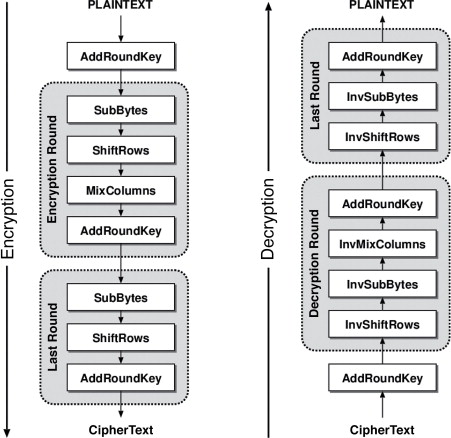
\includegraphics[width=0.90\linewidth]{aes}
   \caption{Ход шифровки/расшифровки блока алгоритмом <<AES>>}
   \label{fig:aes}
\end{figure}
\clearpage

Алгоритм шифрования AES может использоваться в следующих режимах.

\begin{enumerate}
	\item CBC (Cipher Block Chaining) --- режим сцепления блоков;
	\item PCBC (Cipher Block Chaining) --- режим распространяющегося сцепления блоков;
	\item CFB (Cipher Feed Back) --- режим гаммирования с обратной связью;
	\item OFB (Output Feed Back) --- режим обратной связи по выходу.
\end{enumerate}

\begin{figure}[!ht]
   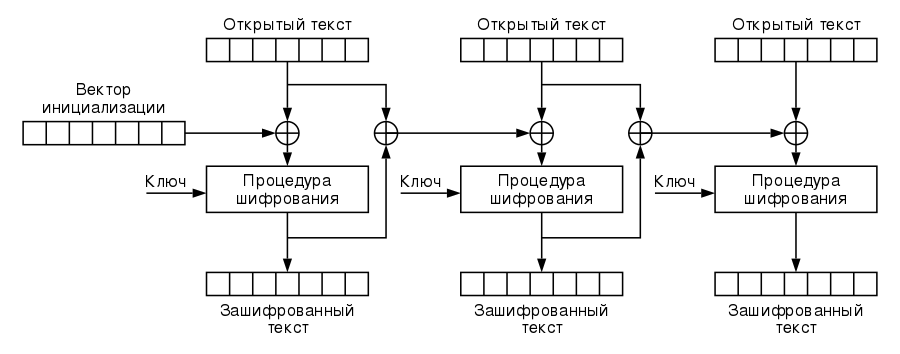
\includegraphics[width=1\linewidth]{pcbc}
   \caption{Ход шифровки/расшифровки сообщения алгоритмом <<PCBC>>}
   \label{fig:pcbc}
\end{figure}

\section*{Заключение}

В ходе работы была разработана программа, осуществляющая шифрование входных данных с помощью алгоритма AES в режиме шифрования PCBC.

%\tableofcontents

%\addcontentsline{toc}{chapter}{Список использованных источников}
%\bibliographystyle{utf8gost705u}
%\bibliography{sources}

\end{document}
